\chapter{AlgTest pyProcess tool}
This chapter describes the development details behind the tool called \texttt{AlgTest pyProcess}, the creation of which was the main goal of this thesis. Its development began as a reimplementation of a tool called \texttt{JCAlgTest Process}. The reasons behind the reimplementation are mentioned in the previous chapter.

The \texttt{AlgTest pyProcess} tool is responsible for the following tasks:
\begin{itemize}
    \item Processing the device profiles generated by automatic testing tools targeted at Trusted Platform Modules and JavaCard smart cards,
    \item Generation of various outputs from these datasets which are primarily tabular and graphical visualizations.
\end{itemize}
\begin{figure}[h]
    \centering
    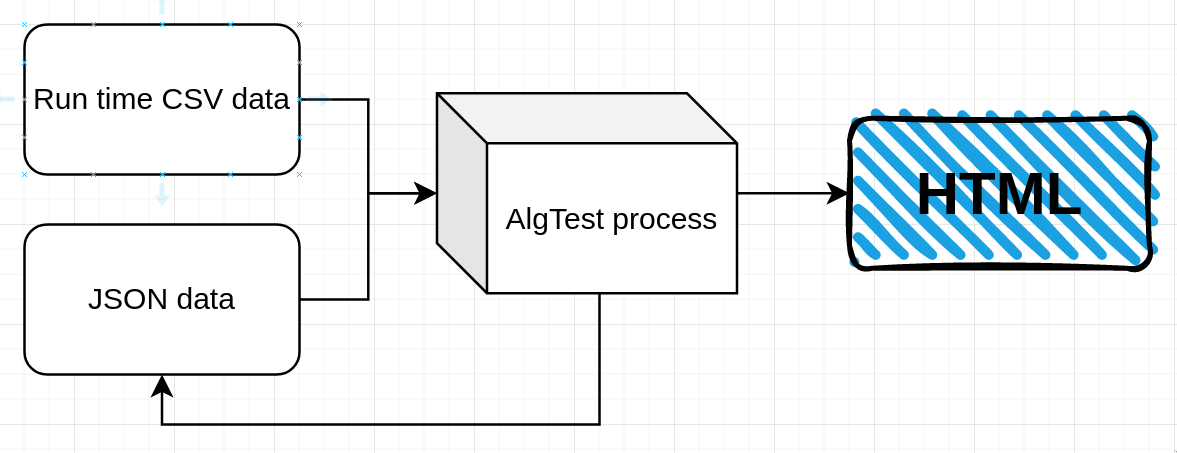
\includegraphics[width=\textwidth]{img/scheme.png}
    \caption{Scheme of AlgTest pyProcess application}
    \label{fig:algtest-process-scheme}
\end{figure}


\section{Parsing}
The \texttt{AlgTest pyProcess} tool is working with datasets that were generated and collected over the years in parallel with the development of the testing tools which generate these datasets. The outputs of these testing tools have been changing over the years too, that is why the testing form of output format for tested devices may differ depending on the version of the testing tool.

There is no prescribed schema for the datasets, but they generally look very similar\footnote{Examples of CSV device profiles are shown in Appendix}. That is why it is convenient to design suitable means of accessing the data contained in them. Such means are provided by mapping these profiles onto class representation. But the first step in order to accomplish that is the parsing of the CSV files which represent the device profiles. 



\section{Results}
The tool produces various visualization and tables as HTML files, which any modern web browser can view. The contents are made responsive and interactive and try to provide convenient means of getting information about the select devices compared to other devices. 

These visualizations may be helpful for various types of audiences:

\begin{itemize}
    \item \texttt{Potential buyers} who want to select their device which suits their needs for supported algorithms or just want to get some insight about the ecosystem, such as what vendors are available. 
    
    \item \texttt{The developers} of software for these devices who want to get the knowledge of the device they are supposed to develop applications for. Insight into the supported algorithms and their performance may enable them to make tailor-made adjustments that may improve the developed application's performance and functionality.
\end{itemize}

The \myref{Table}{table:results} shows the available visualizations for both TPMs and JavaCard smart cards. In the following sections, each result will be described. Several examples of results are shown in the following sections, but some need high resolution to be readable, that is why these examples are also shown in \myref{Appendix}{appendix:diagrams-visualizations}.

\begin{table}[H]
    \begin{adjustbox}{max width=\textwidth}
\begin{tabular}{c|c|c|c|c|c|c|c}
 & Support & Execution time & Similarity & Radar & Heatmap & Comparative & Scalability \\ \hline
Profile & S & P & P & P & C & P & P V \\ \hline
TPM & \cmark & \cmark & \cmark & \cmark & \cmark & \xmark & \xmark \\ \hline
JavaCard & \cmark & \cmark & \cmark & \cmark & \xmark & \cmark & \cmark
\end{tabular}
    \end{adjustbox}
    \caption{Results generated for each device. S means Support device profile, P means Performance device profile, C means cryptographic properties, and P V means variable data length}
    \label{table:results}
\end{table}

\subsection{Support table}
The support table presents the information about the support of particular algorithms and generic information such as vendor information or memory limits for each device.

Support tables for both TPMs and JavaCards contain information extracted from Support device profiles, which are mentioned in \myref{Section}{sec:device-profiles}. All possible algorithms and properties retrieved by the testing tools are put into separate rows, then the profiles are searched. Depending on the existence and contents of the result, an appropriate cell type is shown. 

The table itself may contain up to six types of cells as of now:
\begin{itemize}
    \item Green cell containing 'yes' means algorithm is supported,
    \item Red cell containing 'no' means algorithm is not supported,
    \item White cell containing 'error' means an error was returned, which is generally equivalent to an algorithm not being supported. Hovering over this cell shows the specific error name,
    \item Red cell containing '-' means algorithm or property was not tested or retrieved from the device, similarly as for the error cell, this generally means that the algorithm is not supported
    \item Gray cell contains various numerical or textual values for device properties.
\end{itemize}


%\begin{figure}[H]
%    \centering
%    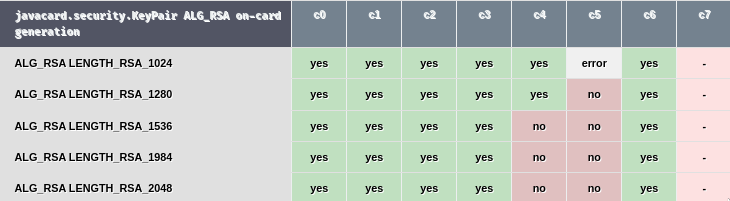
\includegraphics[width=\textwidth]{img/support-table.png}
%    \caption{Support table}
%    \label{fig:support-table}
%\end{figure}

\subsection{Algorithm execution time}
The algorithm execution page presents an alternative to searching in the corresponding raw CSV file representing the Performance device profiles which are mentioned in  \myref{Section}{sec:device-profiles}. 

Firstly, basic information about the device is displayed. Then several tables containing test measurements representing various algorithms with possibly differing configurations are shown. Each table represents a particular category of an algorithm. The table rows generally contain parameters of the algorithm, configuration, operation times, and information about the number of successful or unsuccessful iterations.


\subsection{Similarity table}
The similarity table shows how a chosen pair of devices differ in the performance of selected groups of algorithms. High performance similarity may mean that the pair of devices have a very similar if not identical underlying hardware.

To compute pair similarity, firstly the groups of algorithms need to be selected. Then for each profile, the algorithm operation times have to be normalized, which means they will be scaled to range from 0 to 1 depending on the maximum value across all operation times for a particular algorithm. Then we can compute similarity for pairs of profiles, the measure used is based on the Euclidean distance formula.


\begin{align*}
    d(x, y) = \sqrt{\sum_{i=1}^{n}(x - y)^{2}} 
\end{align*}

Where $x$ and $y$ are normalized operation times for one algorithm supported by both devices, and $n$ is the number of these algorithms. The similarity value is finally computed as $abs(d(x, y) - 1)$, which results in a percentage in the range of 0 to 100.

\begin{figure}[!tbp]
    \centering
    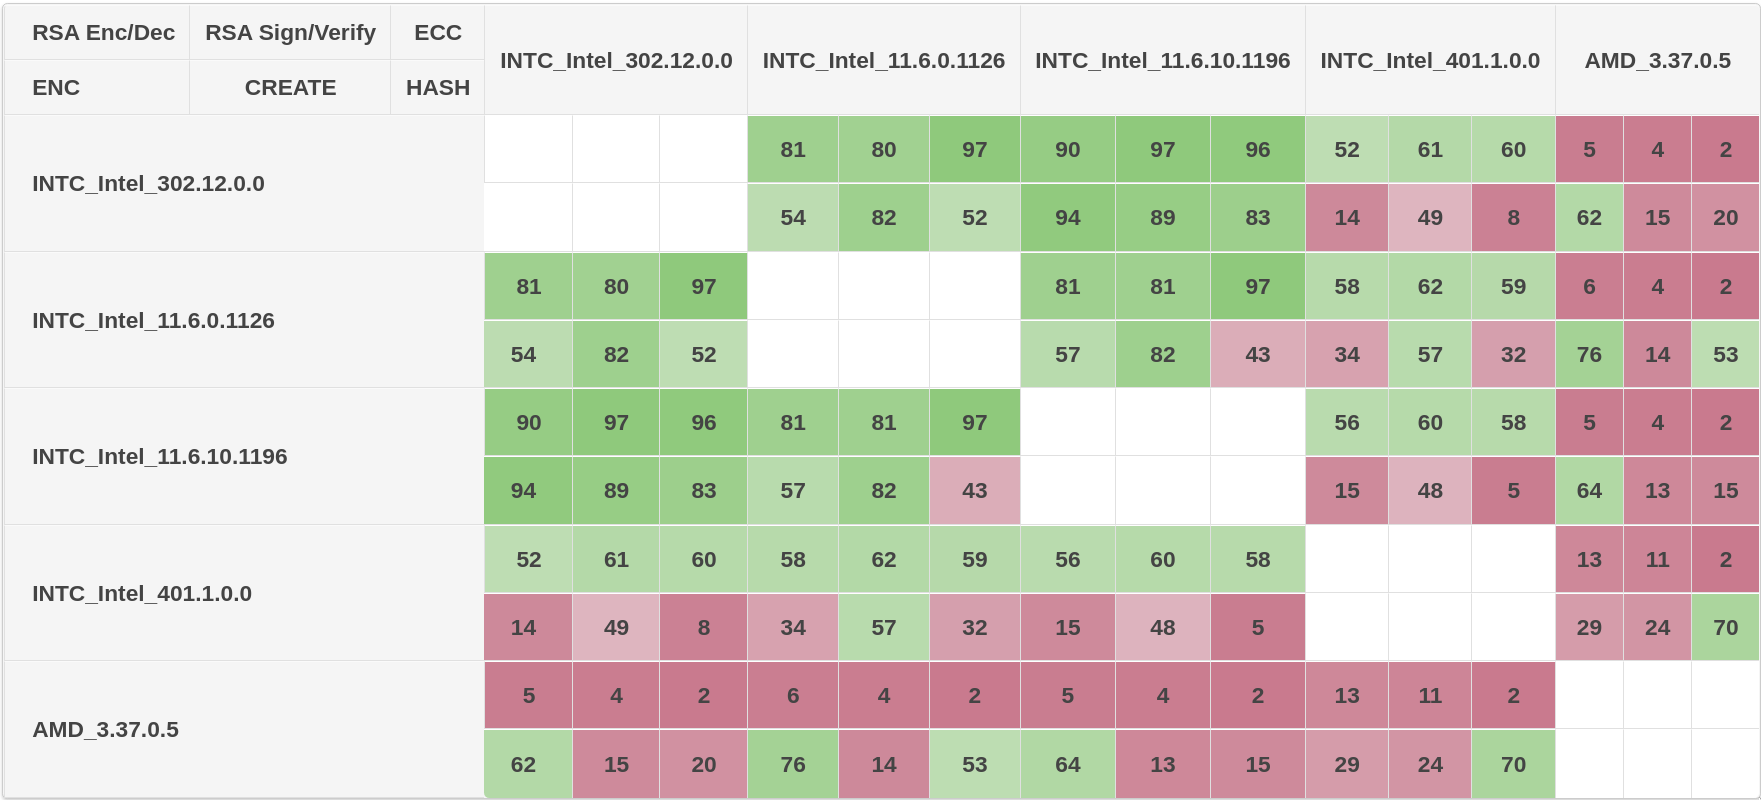
\includegraphics[width=\textwidth]{img/visualizations/tpm-similarity-intext.png}
    \caption{Similarity table comparison of five TPMs. Each cell containing similarity values has either green or red shade which depends on this value. Cells where similarity could not be computed are white.}
    \label{fig:my_label}
\end{figure}


%\begin{figure}[H]
%    \centering
%    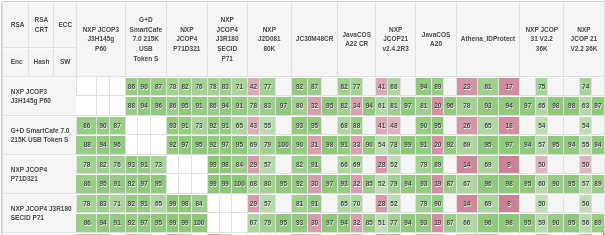
\includegraphics[width=\textwidth]{img/similarity-table.png}
%    \caption{Similarity table}
%    \label{fig:similarity-table}
%\end{figure}


\subsection{Radar graphs}
Radar graphs visualize the device's performance compared to all other tested cards. They can also be used for similarity comparison between two or more devices.

Likewise, as in the case of the similarity table, all algorithm operation times from a selected group need to be normalized. After the normalization, the resulting data is transformed into a JavaScript object compatible with the implementation of Radar chart visualization. Technical details of the tools used are mentioned in \myref{Section}{sec:tools}. The normalized values correspond to percentages, where the closer to 100 percent, the better the device performs compared to other devices. 

\begin{figure}[H]
  \centering
  \subfloat[TPM radar graph]{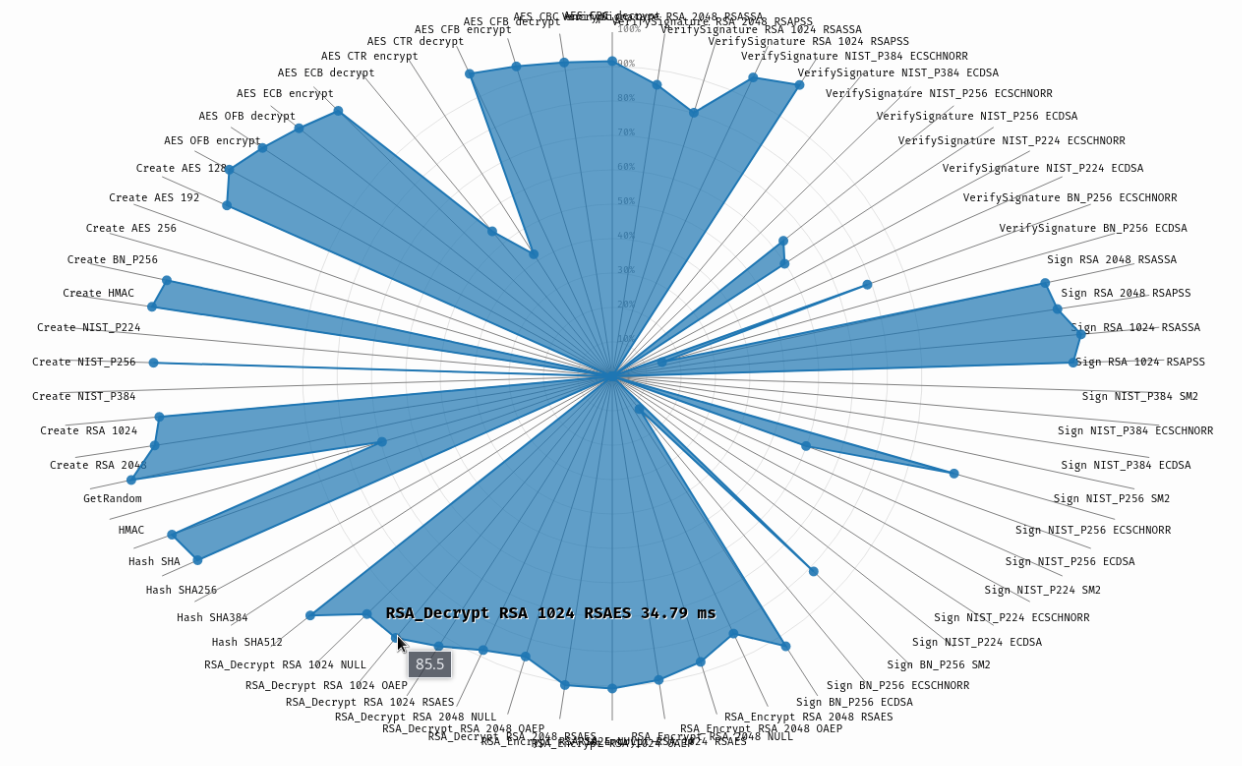
\includegraphics[width=0.48\textwidth]{img/visualizations/INTC_Intel_302.12.0.0 radar graph.png}\label{fig:f1}}
  \hfill
  \subfloat[JC radar graph]{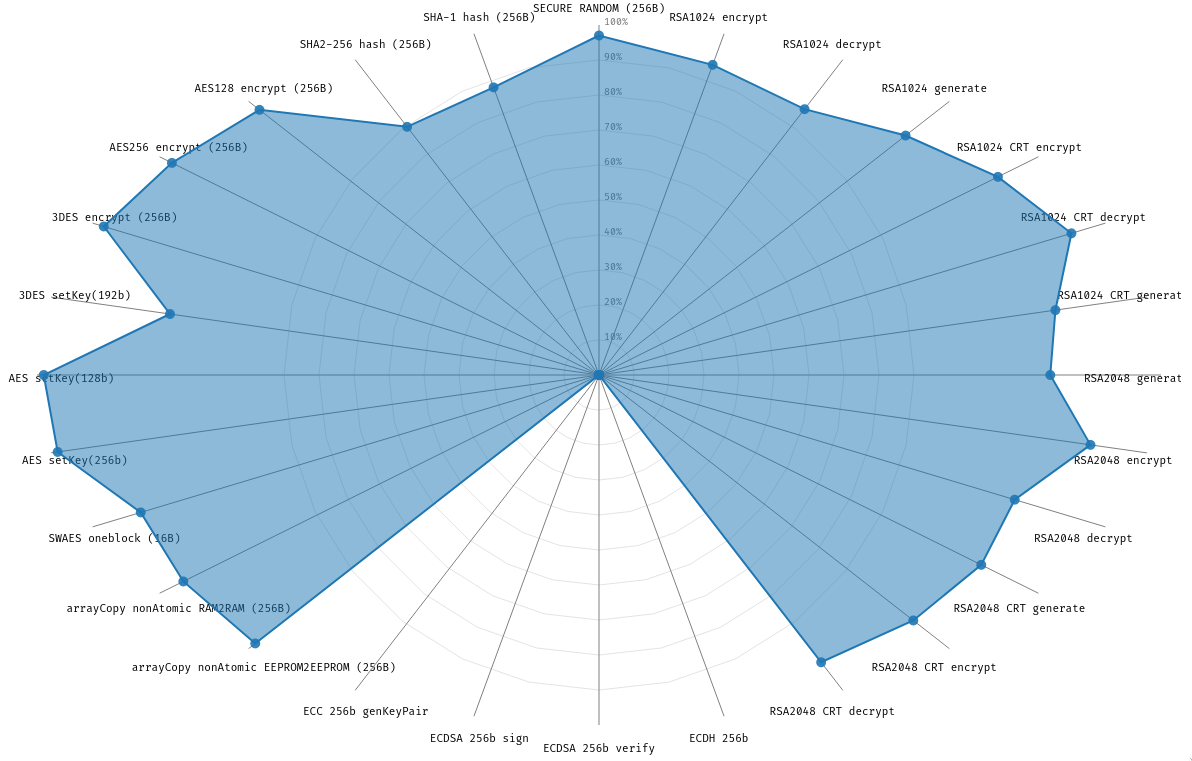
\includegraphics[width=0.48\textwidth]{img/visualizations/JC30M48CR radar graph.png}\label{fig:f2}}
  \caption{Radar graph visualizations.The algorithm identifier with an actual operation time value is shown by hovering over the edge, which is necessary in case there are too many plot axes and their captions overlap each other.}
\end{figure}

\subsection{Heatmap}
Heatmaps can be used in the analysis of generated RSA key pairs. These heatmaps visualize the distribution of most significant bytes (MSB) of RSA private primes $p$ and $q$ and their marginal histograms. The whole chart also contains a separate sub-chart with MSB histograms of these primes $p$ and $q$ and also a histogram of public moduli $n = p \cdot q$. The heatmap for the TPMs may look very sparse, but that entirely depends on the number of generated key pairs.

The motivation behind this chart comes from the research on RSA keys by Švenda et al. \cite{svenda-1mrsa_usenix2016}. They analyzed millions of key pairs generated by almost four dozen software libraries and smart cards. Their analysis revealed, among other things, that depending on the design and implementation of key generation, the origin of the key may be identified just from a public modulus $n$. That is why it may be interesting to analyze the charts that depict primes and moduli distributions for key pairs generated by the TPM devices.

The heatmap chart design is inspired by Nemec \cite{Nemec2016thesis}, but his R script for the generation of the heatmaps could not be easily reused in Python with the TPM datasets, so the plot generation had to be created in Python from the scratch.

\begin{figure}[H]
  \centering
  \subfloat{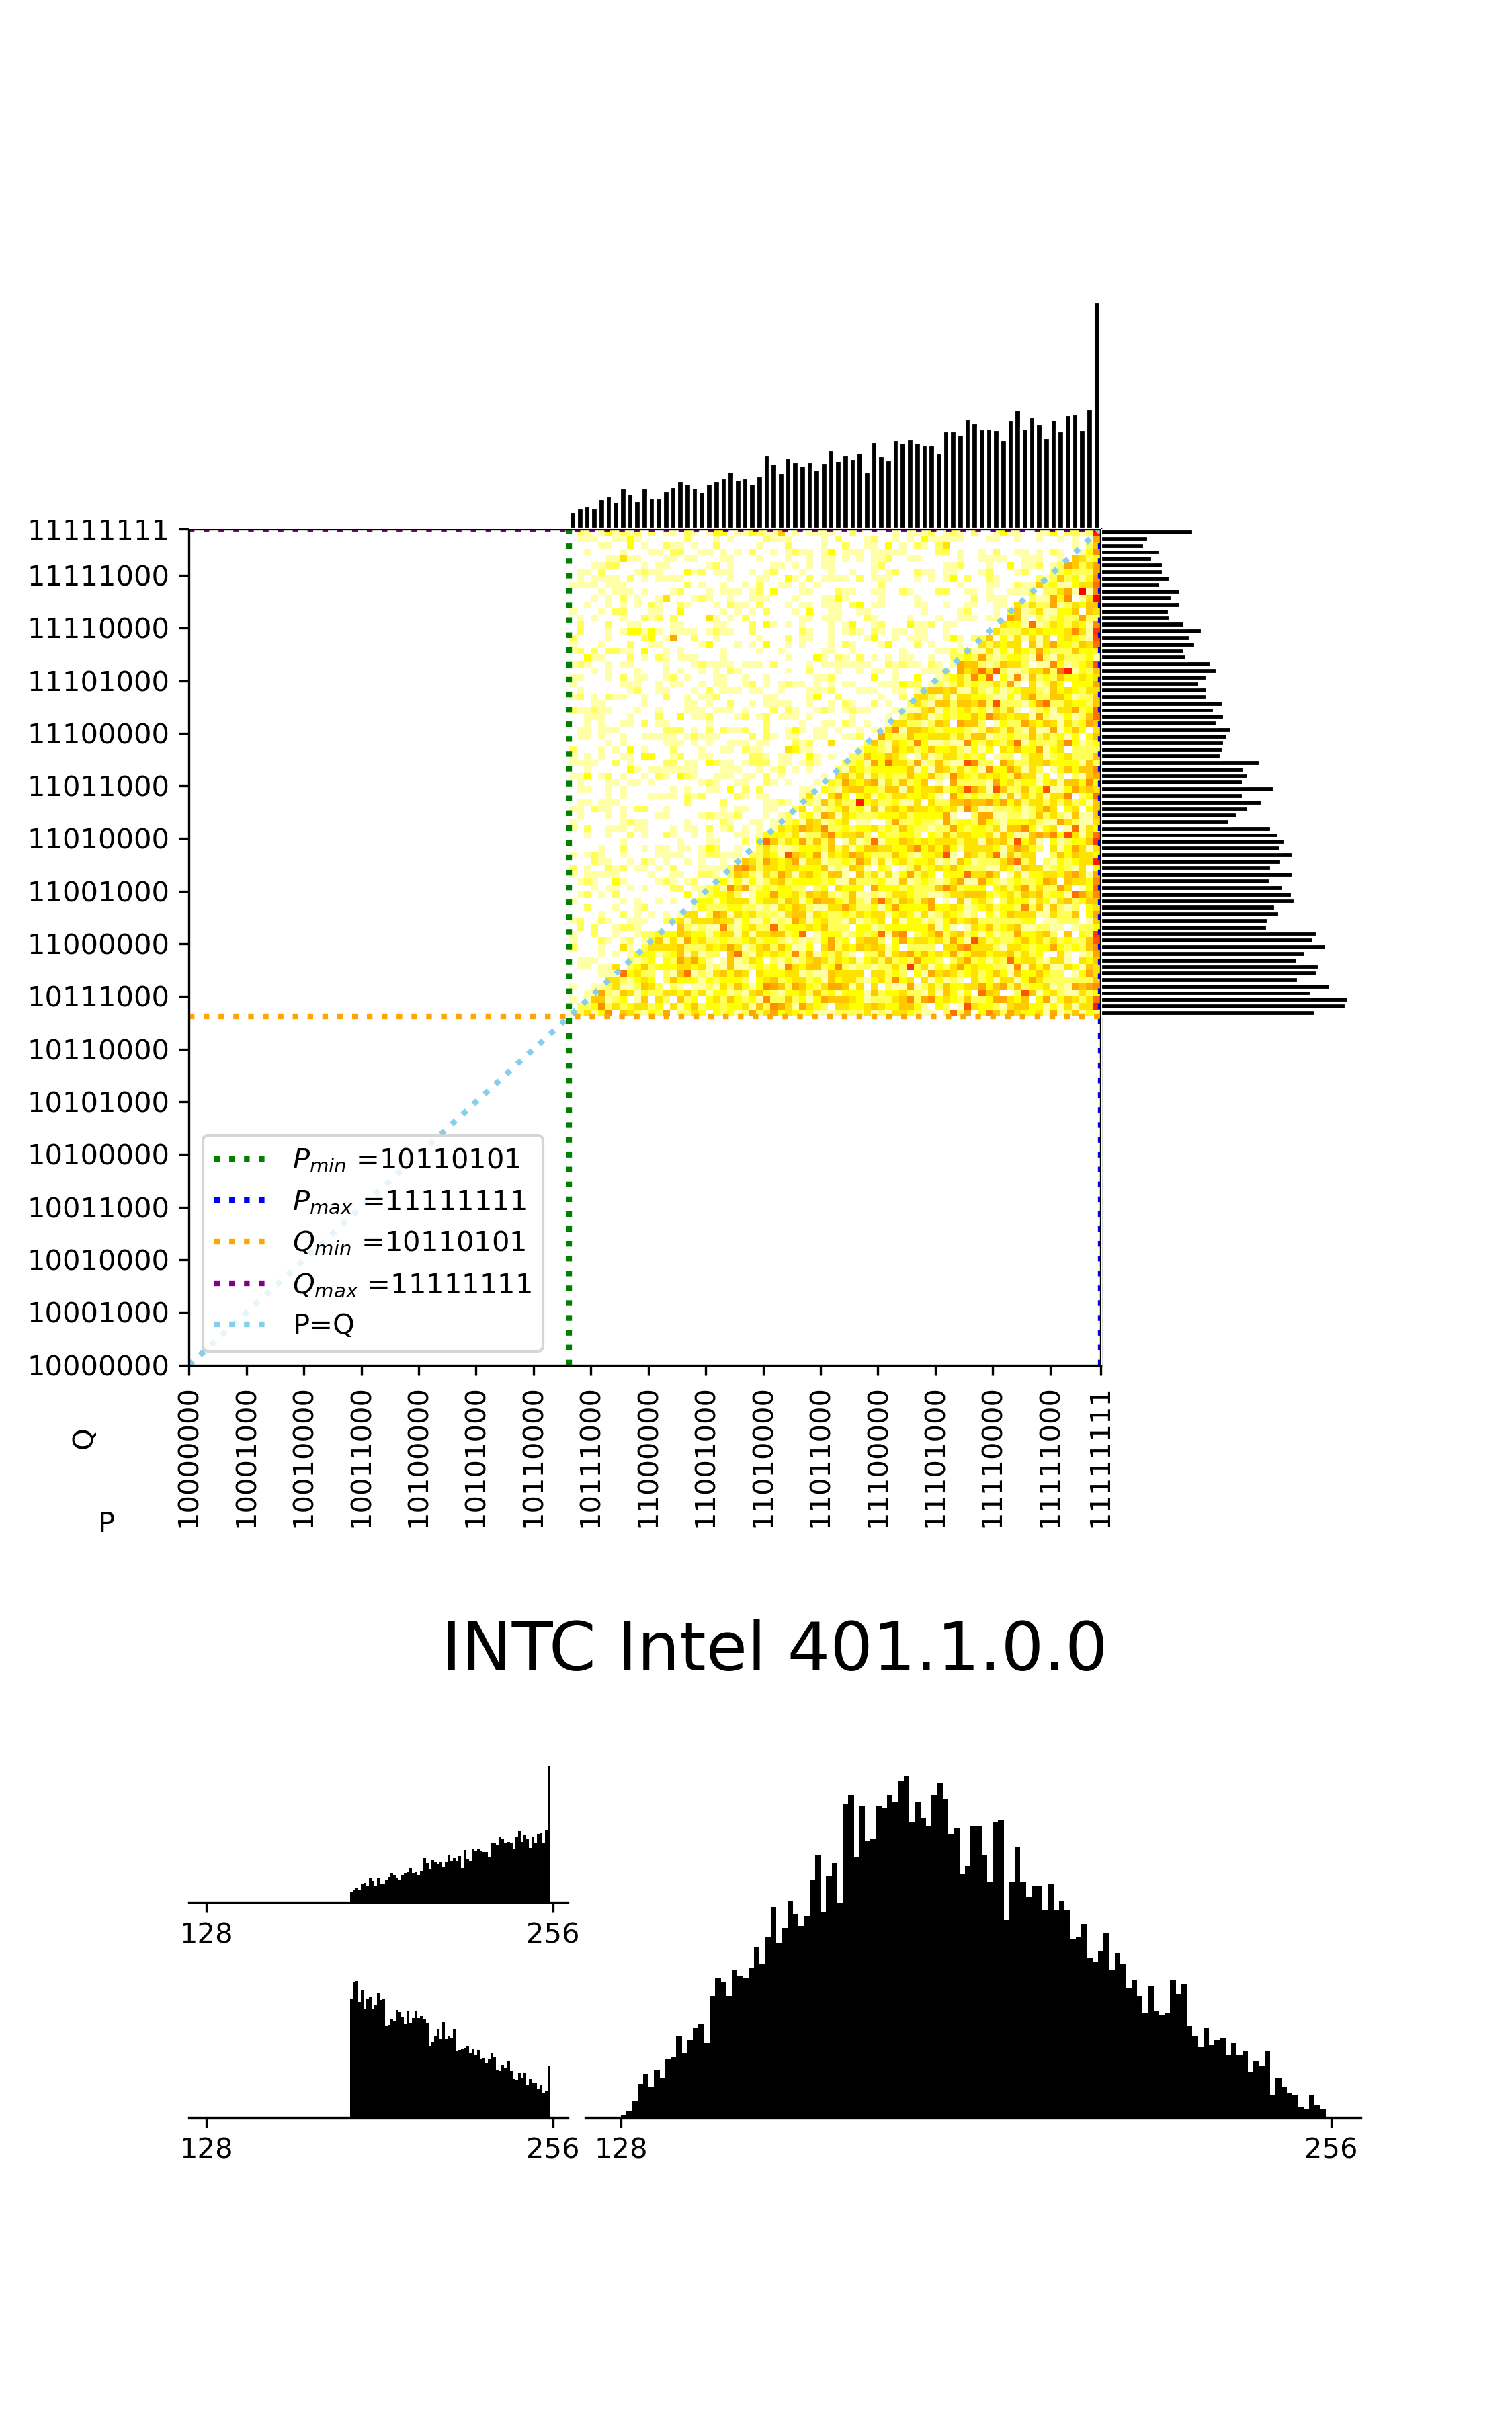
\includegraphics[width=0.48\textwidth]{img/visualizations/rsa.png}\label{fig:f1}}
  \hfill
  \subfloat{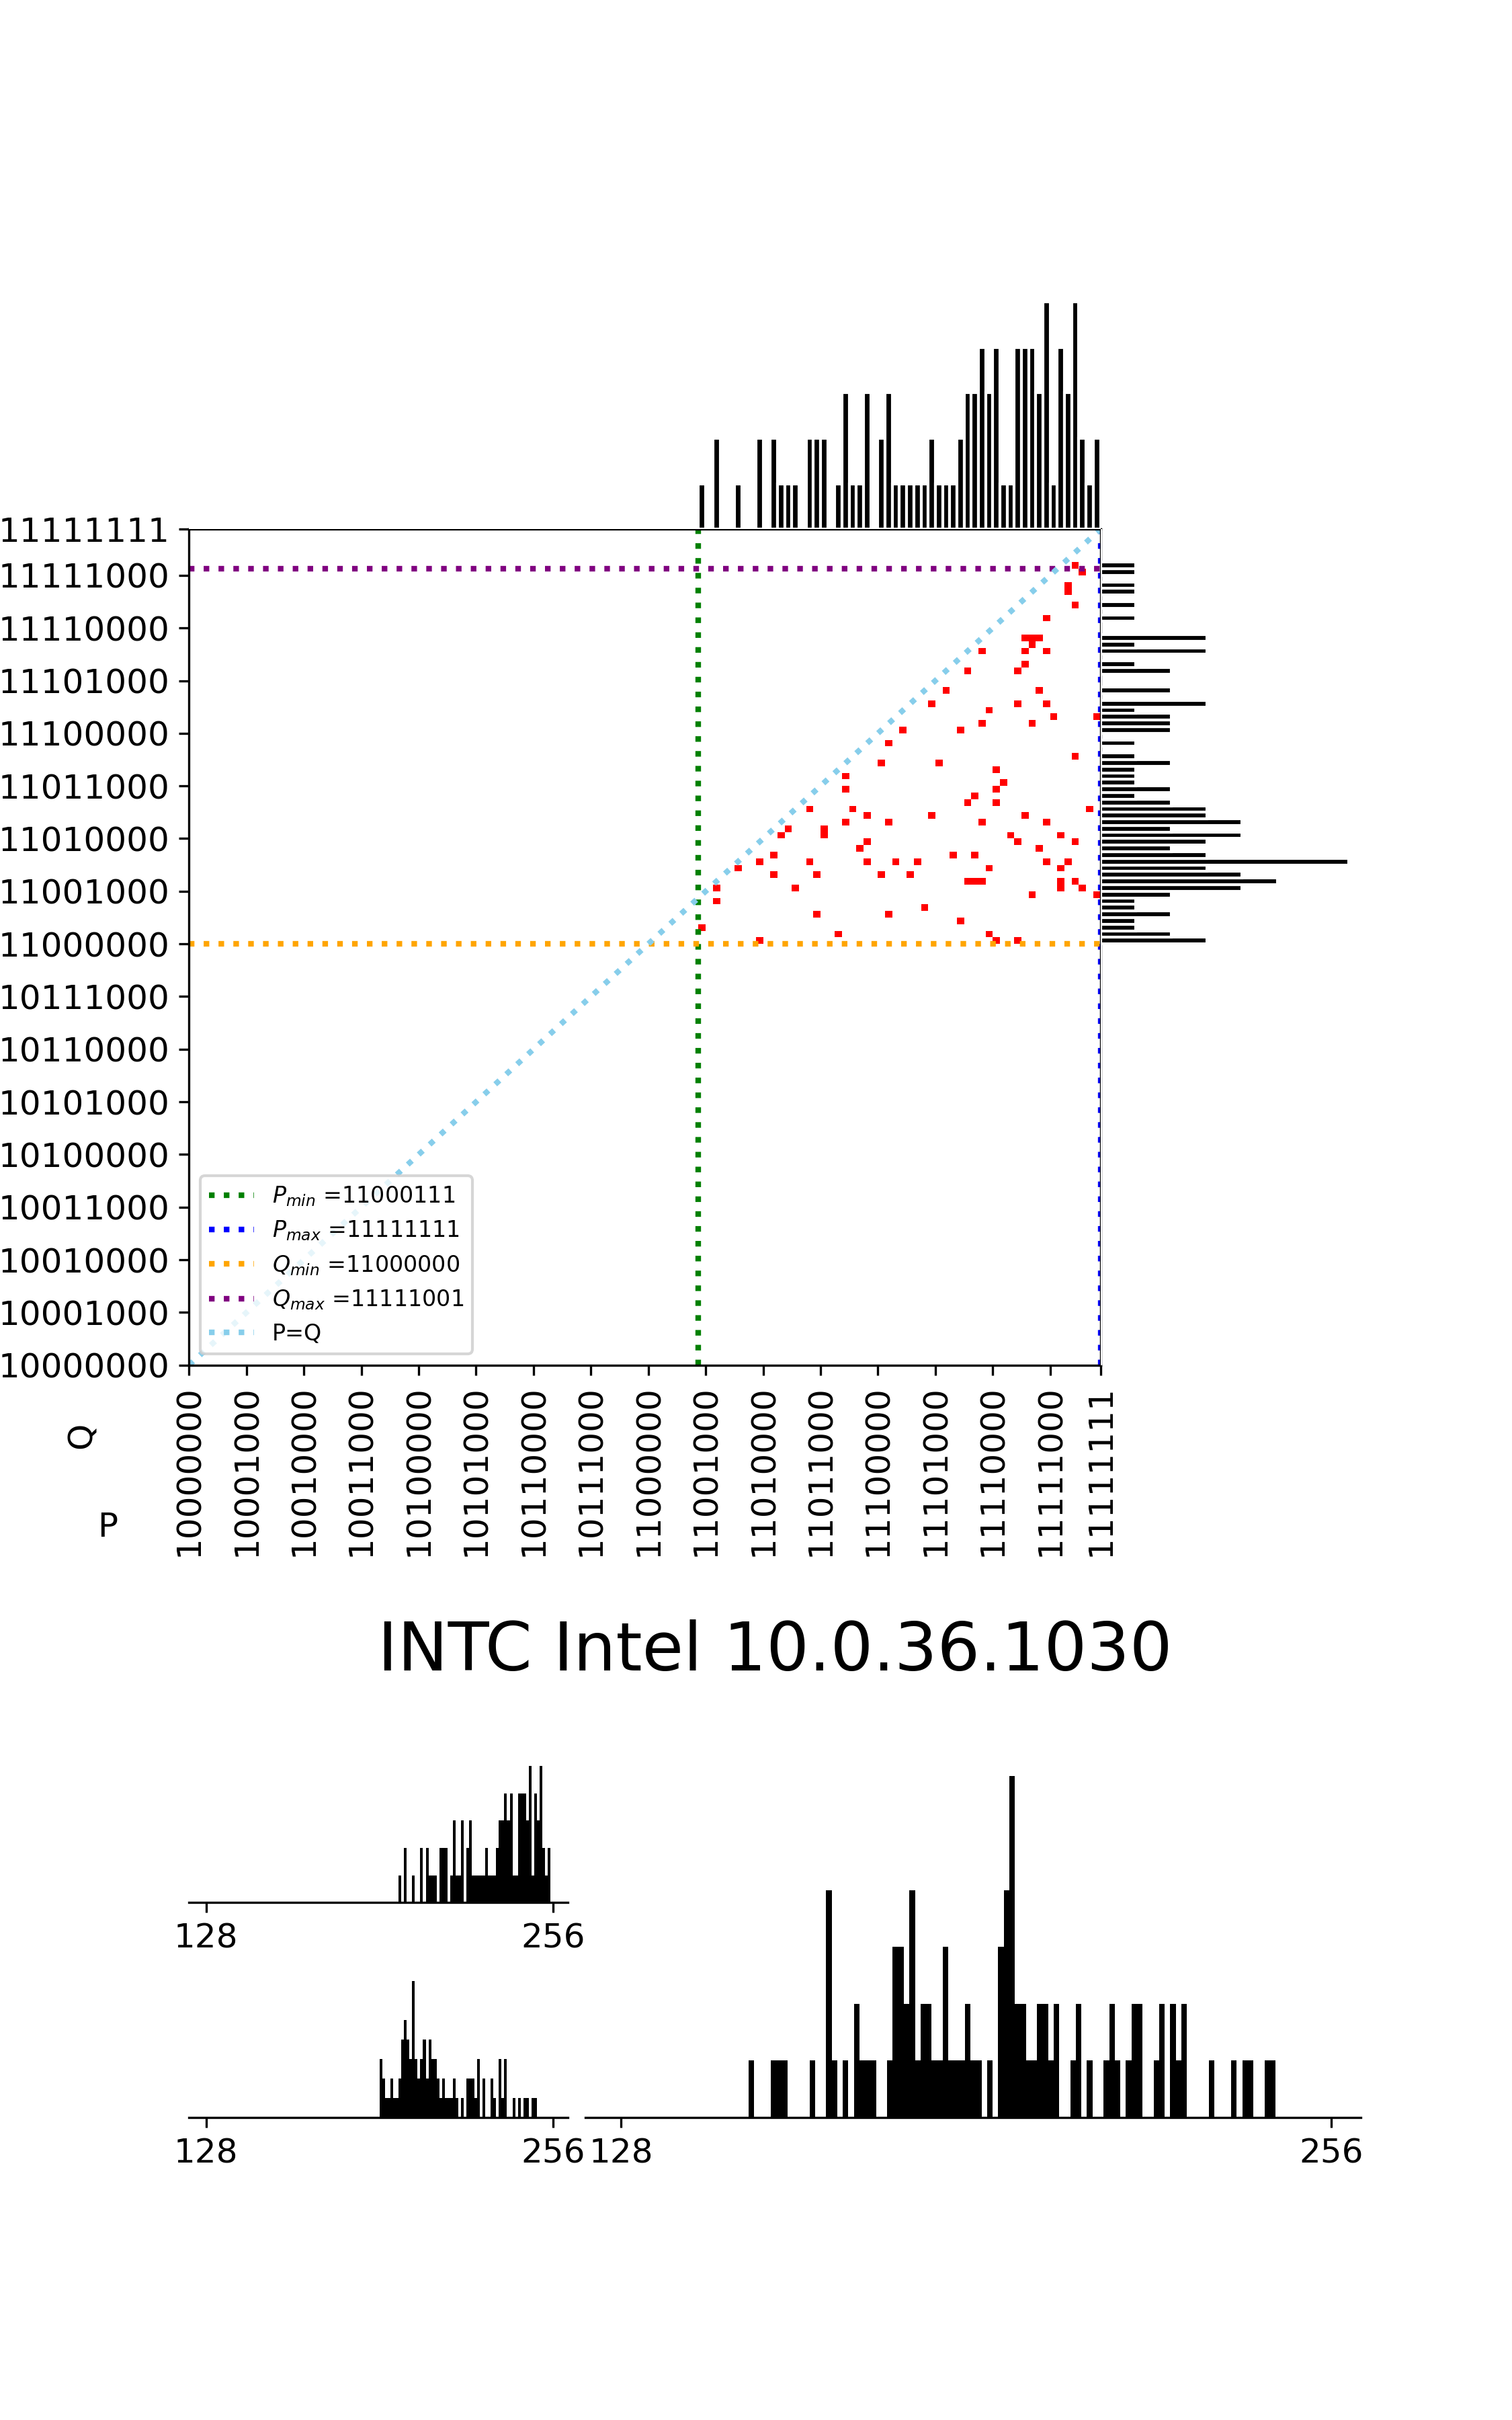
\includegraphics[width=0.48\textwidth]{img/visualizations/rsa1.png}\label{fig:f2}}
  \caption{Heatmaps of two different TPM devices, the left one visualizes ten thousand of RSA 1024-bit keypairs, whereas the right heatmap visualizes only hundred of RSA 2048-bit key pairs}
\end{figure}



%\begin{figure}[H]
%    \centering
%    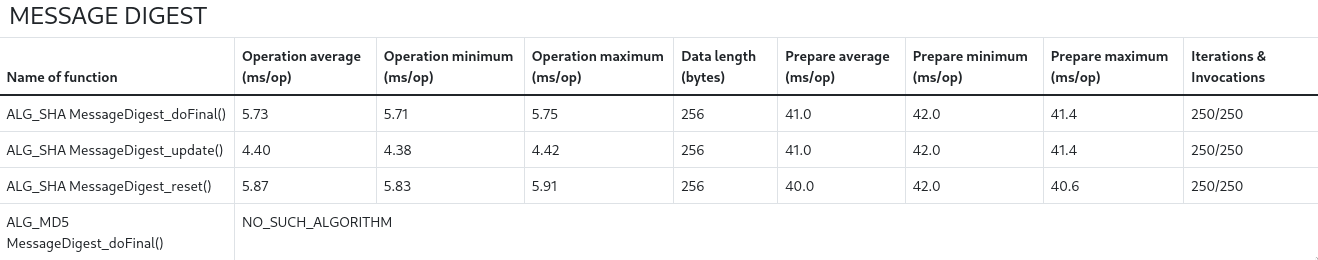
\includegraphics[width=\textwidth]{img/NXP JCOP4 P71D321 execution-time table.png}
%    \caption{Algorithm execution timetable of NXP JCOP4 P71D321}
%    \label{fig:execution-time-table}
%\end{figure}

\subsection{Comparative table}
The comparative table is used for a simple comparison between devices. When generated, the tool creates a page with several tables. Each table represents a category of algorithms whereas each column represents one algorithm from this category. The possible categories can be, for example, asymmetric algorithms, symmetric algorithms, and select frequently used algorithms.

The tables themselves allow for simple sorting according to the column values just by clicking on the selected column according to which rows will be sorted.

%\begin{figure}[H]
%    \centering
%    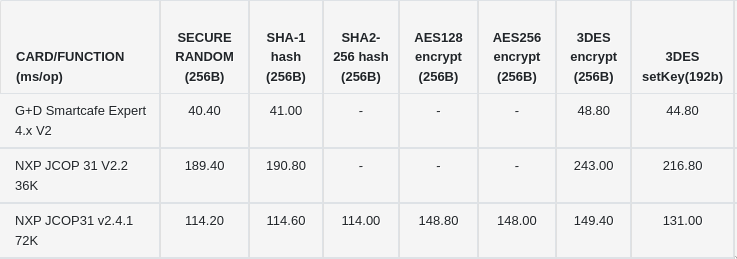
\includegraphics[width=\textwidth]{img/comparative-table.png}
%    \caption{Comparative table}
%    \label{fig:comparative-table}
%\end{figure}

\subsection{Scalability graphs}
Scalability graphs illustrate the device's performance for a specific algorithm depending on input data length. This visualization thus requires variable-length performance results, which are only collected for JavaCards.

One graph is generated for each method that was successfully measured. By hovering over the point in the graph the operation time range of the measurement along with the average operation time are shown.

%\begin{figure}[H]
%    \centering  
%    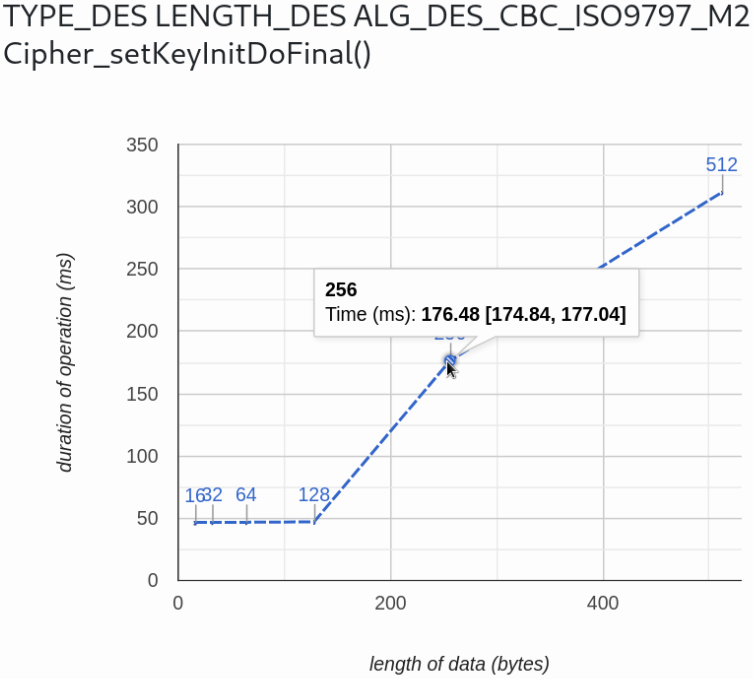
\includegraphics[width=\textwidth-3.5cm]{img/NXP_JCOP_J3D081_v2.4.2R2 scalability graph.png}
%    \caption{
%    Scalability chart of NXP JCOP J3D081 v2.4.2R2 showing performance of DES algorithm in CBC mode, for data lengths We can observe 16, 32, 64, 128 bits the performance seems to be constant, following 256, 512 bits an almost linear increase.
%    }
%    \label{fig:scalability-chart}
%\end{figure}




\section{Tools}\label{sec:tools}
The \texttt{AlgTest process} tool incorporates various instruments to produce desired outputs. As the tool itself is written in Python it is able to utilize various packages from \texttt{PyPI}\footnote{\url{https://pypi.org/}} to aid future extensions.

\begin{itemize}
    \item For creation and manipulation of HTML documents a Python library called \texttt{dominate}\footnote{\url{https://pypi.org/project/dominate/}} is used. Its usage is relatively straightforward, and the code you write is in pure python instead of using additional templating language as in popular web frameworks.
    \item For creation of the heatmaps another Python library called \texttt{matplotlib} was used.
    \item The styling is taken care of by a CSS framework called \texttt{bootstrap}\footnote{\url{https://getbootstrap.com/}} which allows for designing responsive web pages using premade CSS classes and Javascript. The framework itself is extensively used and regularly updated with new versions.
    \item \texttt{Google Charts API}\footnote{\url{https://developers.google.com/chart}}  is utilized for Scalability graph visualisation.
    \item \texttt{D3.js library}\footnote{\url{https://d3js.org/}}  is used for visualisation of Radar graphs.
\end{itemize}

